\subsection{实验设计与执行完整性}
冻结 LightGBM、TabM、XGBoost 各三个种子，共9个评分器。沿用原数据划分与阈值策略族，验证集30751人，测试集61503人。评分模型没有重新训练；所有新权重在验证集拟合并序列化之后才读取测试标签。原测试集在历史研究中已经查看过，不能称为新的盲测。

run005：收益预算0.5\%/1\%/3\%，比较绝对 maxmin、归一化 maxmin 与完整 leximin，保留99行记录（含收益及旧方法对照）。run006：固定收益预算1\%，额外伤害预算0.1/0.3个百分点，同样三个目标，保留72行记录。主比较预先指定为0.1个百分点，没有从测试结果选预算。

另对9个评分器设置0.05/0.10/0.20个百分点三个机会改善目标，完成27个验证集逆向定价问题。61项单元测试通过；run006的4977项独立重放及指标检查通过。独立业务审计与归一化水位审计分开记录。

\subsection{严格最低伤害集合：没有实际分配空间}
主收益预算下，54个群体跨度最大仅为0.0001544个百分点，中位约0.00000519个百分点。9个配置中4个全部坐标低于固定范围容差。27个严格 leximin 策略中，3个归一化数值认证未通过（均 LightGBM seed731），尽管原尺度的业务约束满足；这些失败已保留。不能把退化集合上的归一化数值放大当作新收益。

0.5\%至3\%三个预设收益预算下，各评分器的最低伤害相同；主设置收益约束的局部对偶价格均为0。此时多牺牲一点收益不是减少最低必要伤害的有效杠杆。这个结论仅针对已检查的预算区间、风险条件和策略族。

\begin{figure}[htbp]\centering
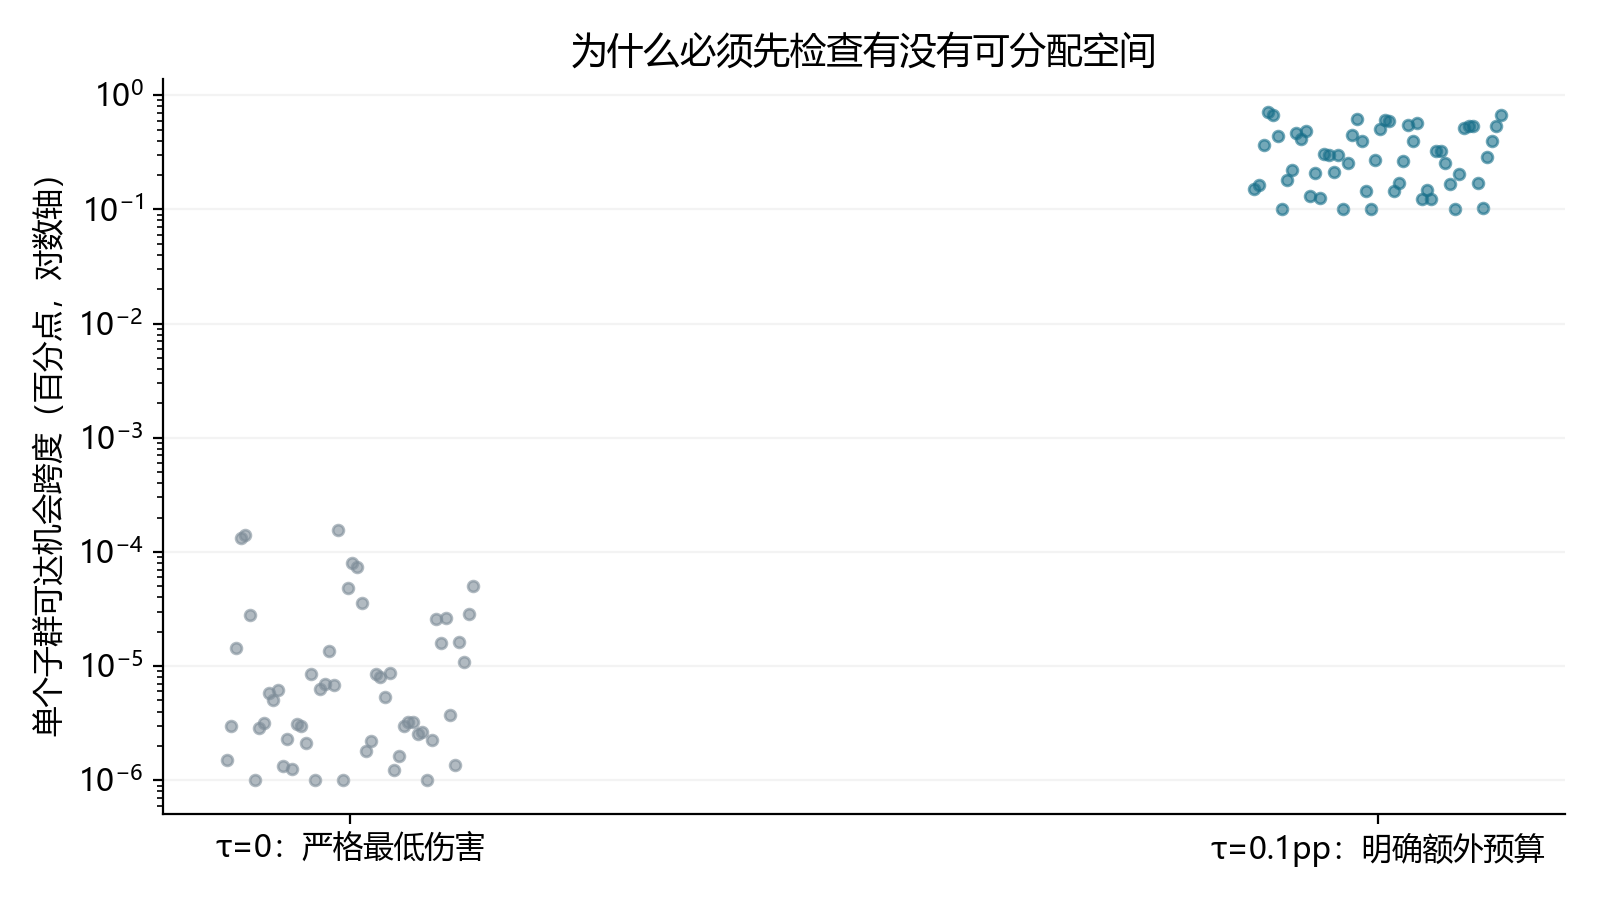
\includegraphics[width=.9\linewidth]{images/allocation_space.png}
\caption{业务可分配空间与数值退化。每种设置54个子群观测。}\end{figure}

\subsection{归一化分配是不同取舍，不是全面改进}
正预算下63条策略记录（9条收益基准、54条新分配规则）业务审计通过，18个完整 leximin 均通过归一化水位审计，无退化维度。所有18个配置中，完整 leximin 与一次归一化 maxmin 的实际结果在数值精度内相同；完整理论避免一般情况下的遗漏，但此次数据没有显示额外收益。

LightGBM 三种子测试均值如下，双预算均为1\%收益、0.1个百分点额外损害：
\begin{center}\small
\begin{tabular}{lrrrr}\toprule
方法 & 情景贡献 & 宏观差距pp & 最差误拒\% & 基准伤害D(pp)\\\midrule
旧绝对最弱组目标 & 35770.98 & 1.219 & 18.337 & 1.229\\
归一化机会目标 & 35786.89 & 1.475 & 18.548 & 1.155\\\bottomrule
\end{tabular}\end{center}
新目标贡献增加约15.91单位，最大附带损害降低约0.074个百分点，但最差群体误拒增加约0.211个百分点。更重要的是，单种子2pp宏观差距目标：新目标仅2/9个评分器满足，旧目标为5/9；LightGBM分别为1/3与3/3。均值不能掩盖个别配置超限。所有9个主配置的测试风险与收益底线仍满足。

因此不以归一化 leximin 直接替换已有主审批方法。它适合成为资源分配视角下的可解释对照，核心研究贡献进一步集中到双预算约束诊断与逆向机会价格。

\begin{figure}[htbp]\centering
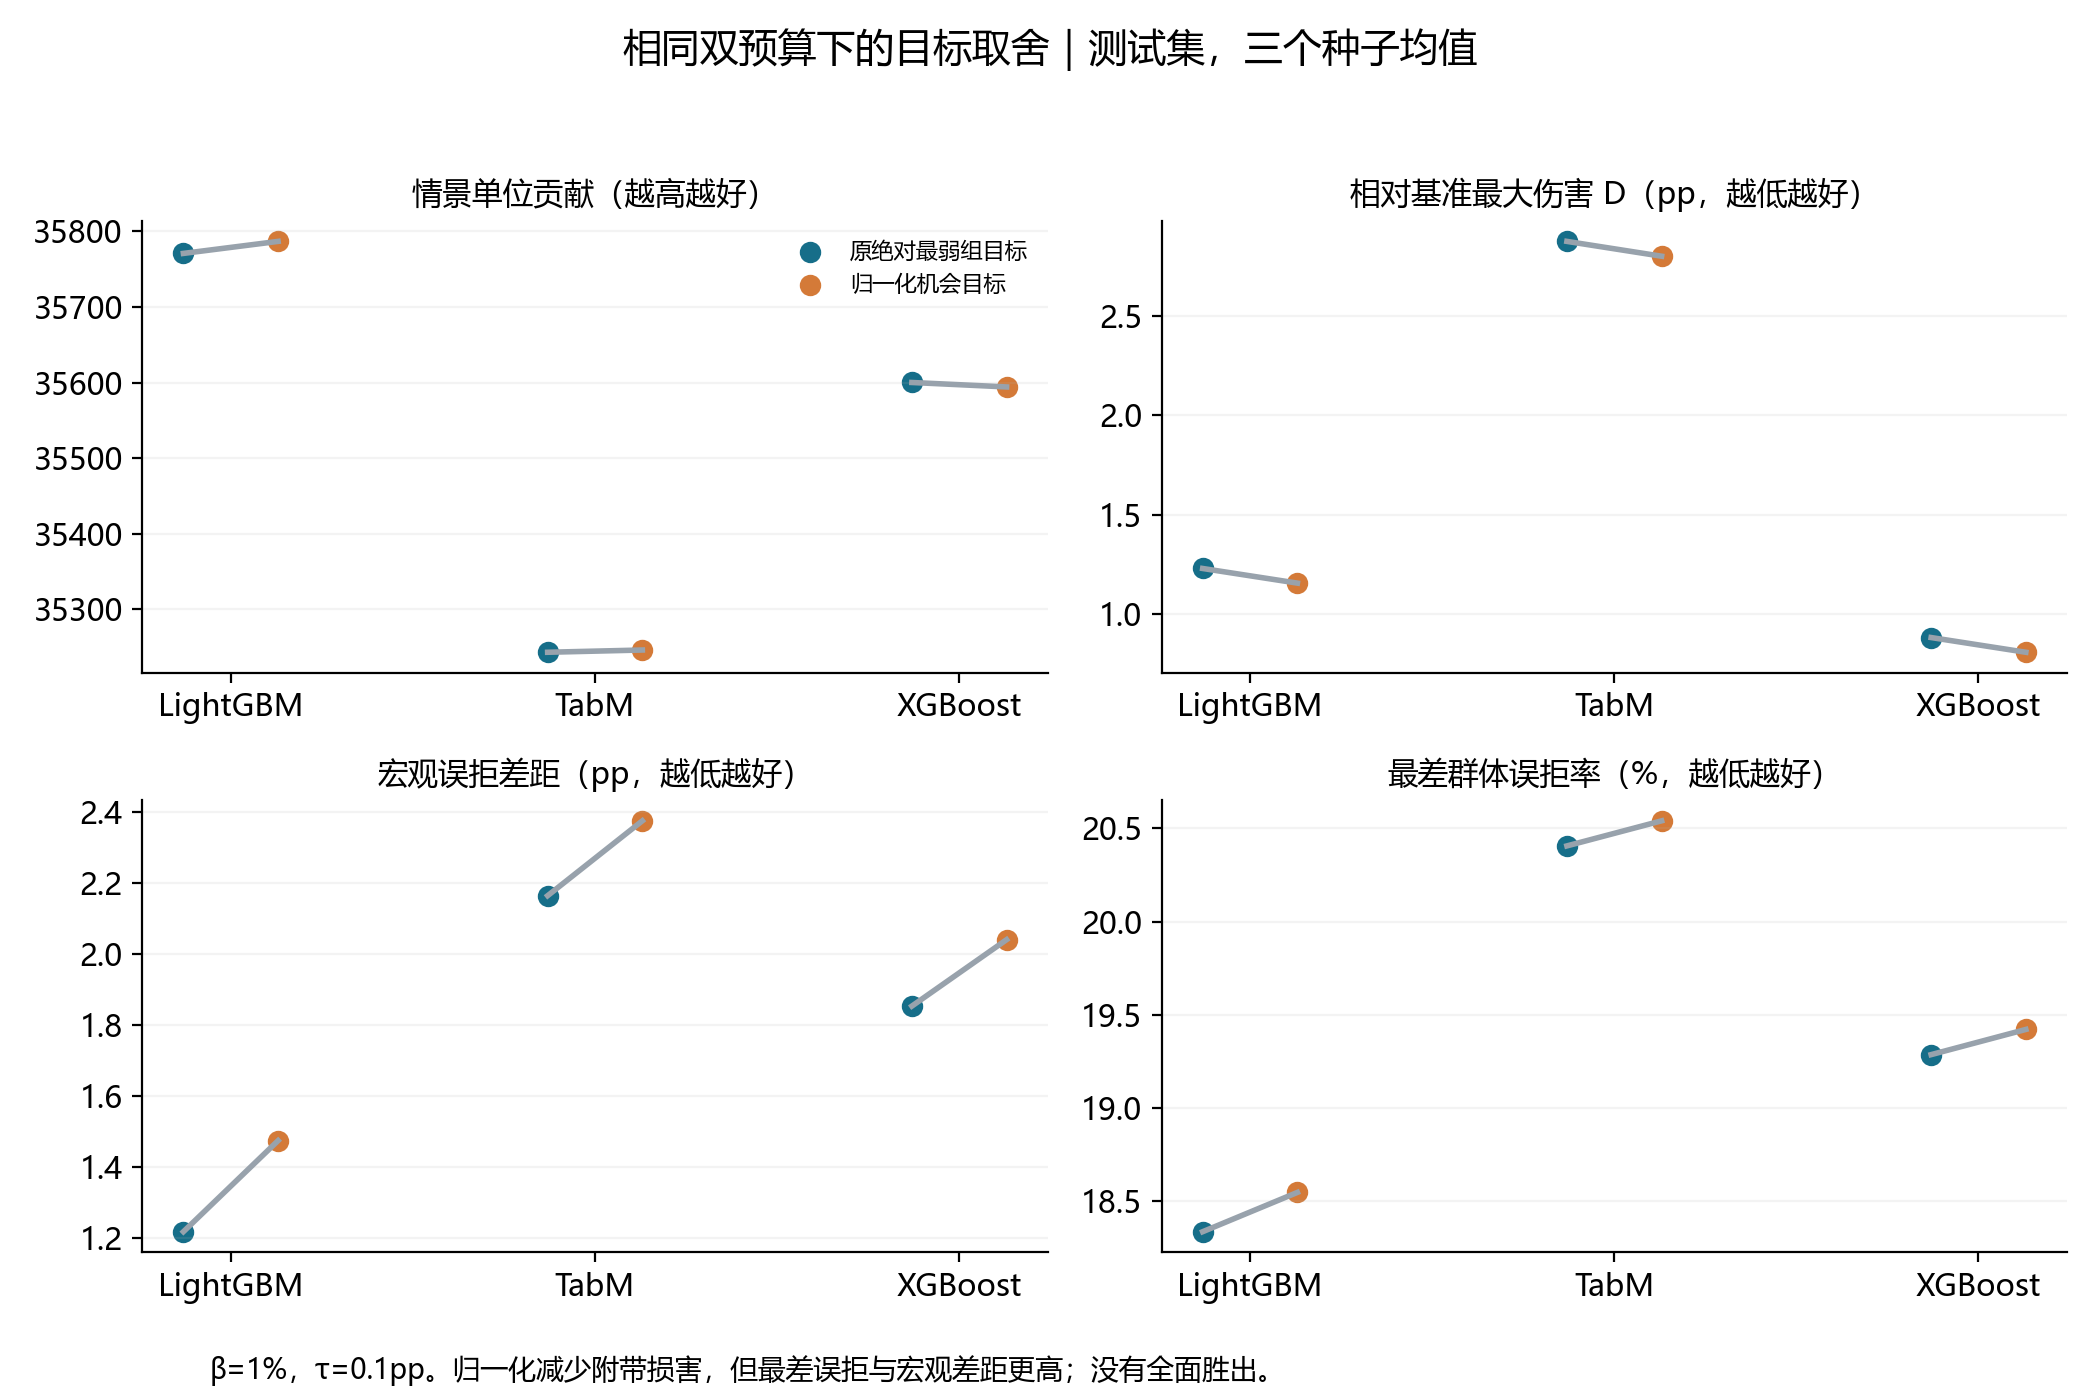
\includegraphics[width=\linewidth]{images/same_budget_tradeoff.png}
\caption{相同预算下三个模型的取舍，全部三个种子保留。}\end{figure}

\subsection{逆向机会定价：直接回应业务目标}
27个预设目标在验证集均可行，目标、风险、资金、收益及最低伤害价格均经重放检查。LightGBM三个种子的平均结果为：
\begin{center}
\begin{tabular}{rrr}\toprule
最弱机会底线提高pp & 最低额外伤害预算pp & 相对收益基准贡献变化\%\\\midrule
0.05 & 0.01589 & -0.1149\\
0.10 & 0.03643 & -0.1188\\
0.20 & 0.07753 & -0.1266\\
\bottomrule\end{tabular}\end{center}
这是最低保护价格，不是以人民币计价的利润损失；右列另报告情景贡献变化。每个目标的策略是在达到最低价格后再最大化贡献。均值之外，原始逐种子表与全部混合权重也已保存。

例如 LightGBM seed731：严格保护下最弱正常客户机会为80.119842\%，最低必要伤害为1.588621个百分点。要求共同机会底线提高0.10个百分点时，最低再允许0.022142个百分点额外伤害，得到相对收益基准约0.208968\%的贡献损失、5\%的风险。总损害上限约为1.610763个百分点，不应只报较小的额外部分。

\begin{figure}[htbp]\centering
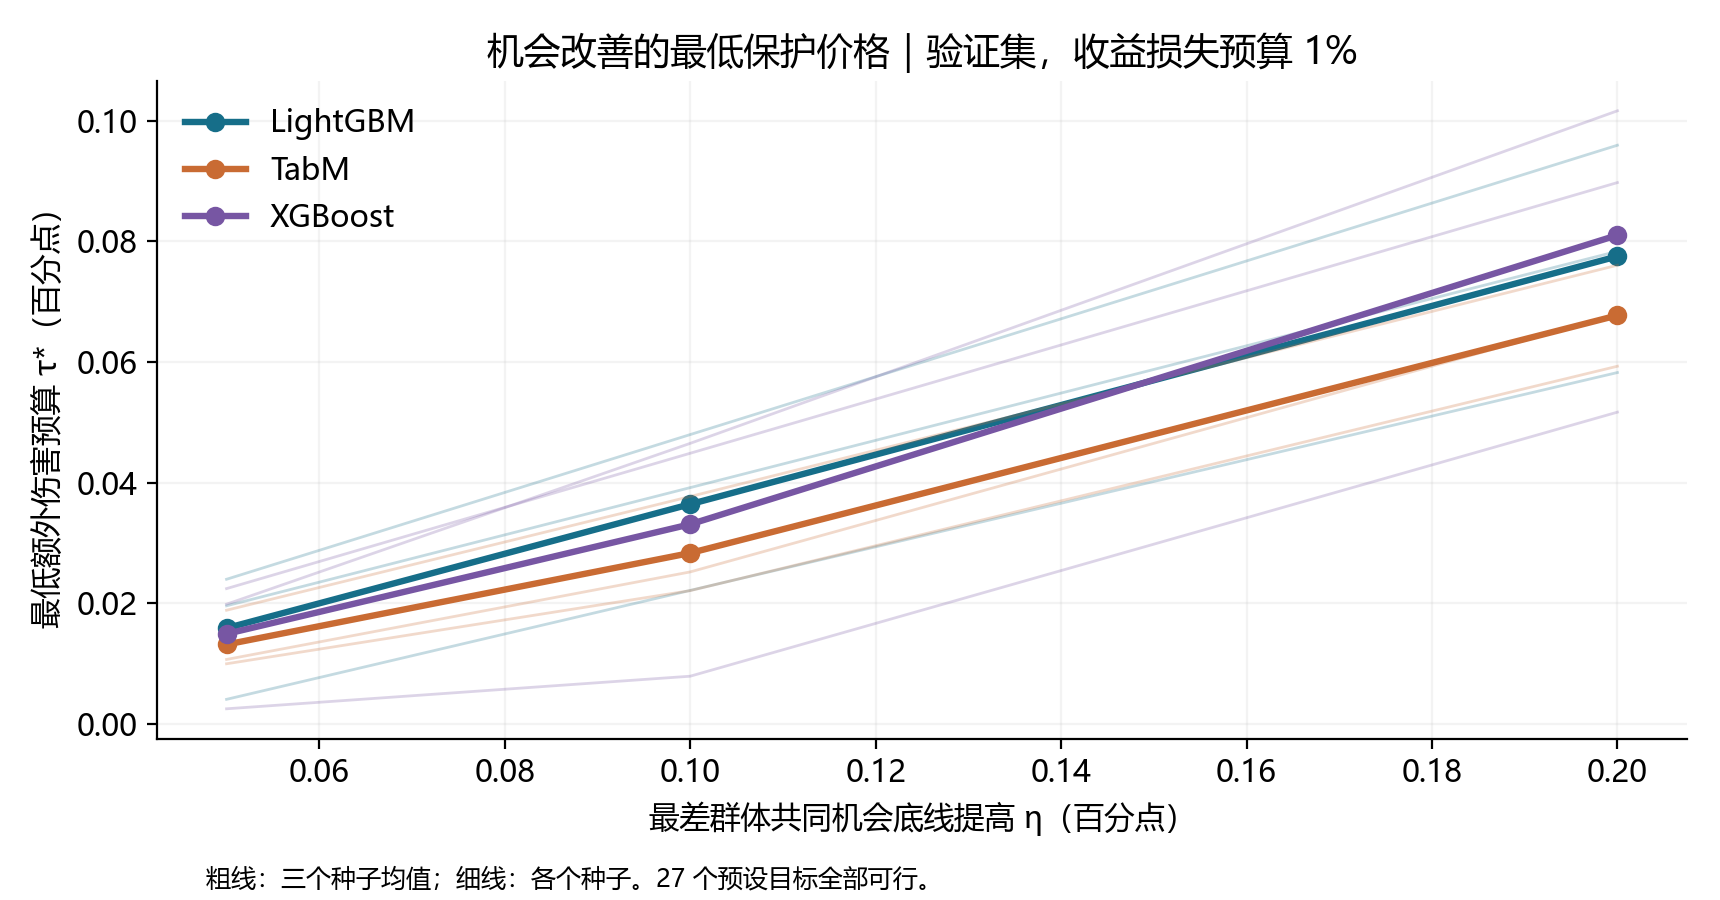
\includegraphics[width=.95\linewidth]{images/inverse_opportunity_price.png}
\caption{预设改善目标的最低额外保护价格。}\end{figure}

\subsection{冻结逆向定价策略的测试回放}
全部27个已保存策略随后在同一测试集重放，没有重新拟合或挑选目标。2160项独立检查通过；风险与收益底线27/27满足，2pp宏观差距仅8/27满足。相对各自冻结的严格保护W0策略，最差群体机会23/27提高，但只有9/27达到完整的预设提高幅度。因此，验证集逆向价格不能解释成未来样本的确定兑现保证。

LightGBM三个种子平均：预设提高0.05/0.10/0.20个百分点时，测试实际最差机会分别提高约0.0421/0.0922/0.1923个百分点。这里比较两个冻结策略在测试集上的最差机会之差，和验证集的绝对门槛 $W_0+\eta$ 区分记录。原始目标、未达标策略和收益变化全部保留在 \texttt{opportunity\_prices/test\_evaluation.csv}。

项目汇报应把双预算与逆向定价作为业务分析贡献，把原绝对最弱组方法继续作为当前表现较稳定的审批参考。这不依赖将新分配目标包装成全面性能升级。

\subsection{文件与复现}
实现位于 \texttt{research\_extension\_v3/theory\_extension}；本说明所在目录为 \texttt{theory\_note}。原始新结果位于 \texttt{results/run\_005\_theory} 与 \texttt{results/run\_006\_budget}，逆向定价位于后者的 \texttt{opportunity\_prices}。策略、配置、源代码快照或哈希、检查结果、配对区间、统计证书和原始图表均保留。原 run001--004 未改动。
